\iffalse
\documentclass[12pt]{article}
\usepackage{graphicx}
\usepackage[none]{hyphenat}
\usepackage{graphicx}
\usepackage{listings}
\usepackage[english]{babel}
\usepackage{graphicx}
\usepackage{caption} 
\usepackage{hyperref}
\usepackage{booktabs}
\usepackage{array}
\usepackage{amsmath}   % for having text in math mode
\usepackage{extarrows} % for Row operations arrows
\usepackage{listings}
\lstset{
  frame=single,
  breaklines=true
}
  
%Following 2 lines were added to remove the blank page at the beginning
\usepackage{atbegshi}% http://ctan.org/pkg/atbegshi
\AtBeginDocument{\AtBeginShipoutNext{\AtBeginShipoutDiscard}}


%New macro definitions
\newcommand{\mydet}[1]{\ensuremath{\begin{vmatrix}#1\end{vmatrix}}}
\providecommand{\brak}[1]{\ensuremath{\left(#1\right)}}
\providecommand{\norm}[1]{\left\lVert#1\right\rVert}
\newcommand{\solution}{\noindent \textbf{Solution: }}
\newcommand{\myvec}[1]{\ensuremath{\begin{pmatrix}#1\end{pmatrix}}}
\let\vec\mathbf

\begin{document}

\begin{center}
\title{\textbf{Properties of Triangles}}
\date{\vspace{-5ex}} %Not to print date automatically
\maketitle
\end{center}
\setcounter{page}{1}

\section{10$^{th}$ Maths - Chapter 7}
This is Problem-3 from Exercise 7.1
\begin{enumerate}
\item Determine if the points $(1,5), (2,3), \text{ and } (-2,-11)$ are collinear.  \\
	\fi
\solution 
 We know that points $\vec{A}, \vec{B} \text{ and } \vec{C}$ are collinear, if
\begin{align}
  \label{eq:10/7/1/31}
\text{rank}\myvec{ 
	\vec{A}^\top \\ 
	\vec{B}^\top \\ 
	\vec{C}^\top 
}    &=  1 
\end{align}
Since
\begin{align}
	\myvec{ \vec{A}^\top \\ 
			\vec{B}^\top \\ 
			\vec{C}^\top 
} =   		\myvec{
        		1 & 5 \\
        		2 & 3 \\
        		-2 & -11 
}
\\
\xleftrightarrow[{R_3\rightarrow R_3+2R_1}]{{R_2\rightarrow R_2-2R_1}}  \myvec{
  1 & 5 \\
  0 & -7 \\
  0 & -1 
}    
\xleftrightarrow[]{{R_3\rightarrow R_3-\frac{1}{7}R_2}}  \myvec{
  1 & 5 \\
  0 & -7 \\
  0 & 0 
},
\end{align}
 the rank of the matrix is 2. From \eqref{eq:10/7/1/31}, the points are not collinear.  This is verified by Fig.  
 \ref{fig:10/7/1/3Fig1}, where the given points constitute a triangle and not a line.
\begin{figure}[!h]
	\begin{center}
		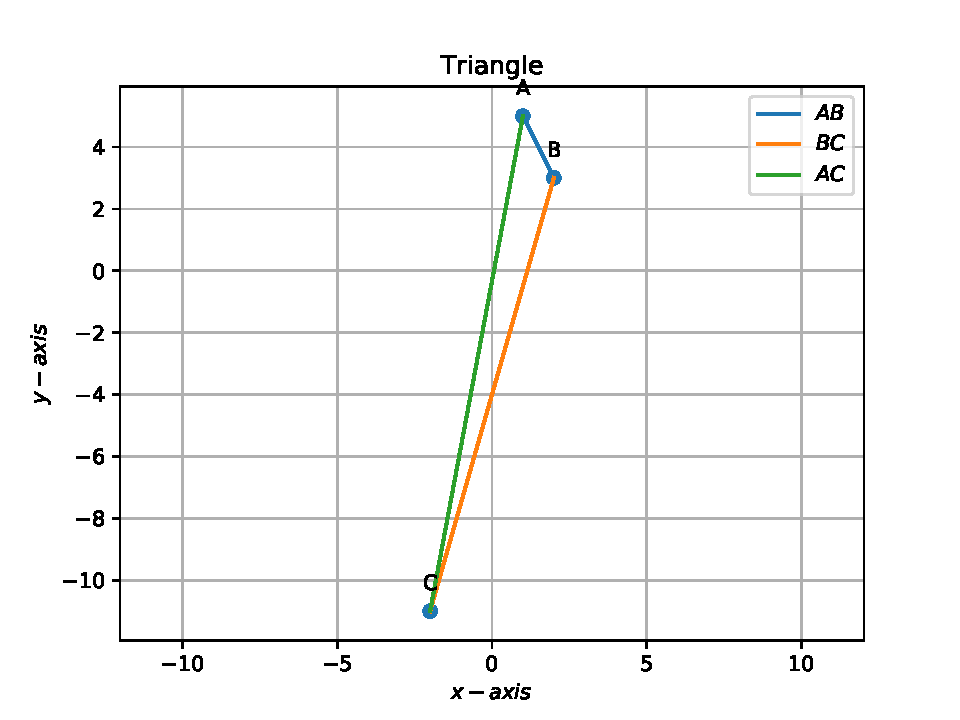
\includegraphics[width=\columnwidth]{chapters/10/7/1/3/figs/problem3.pdf}
	\end{center}
\caption{}
\label{fig:10/7/1/3Fig1}
\end{figure}

